This section illustrates the end-to-end sequences that span multiple services and the edge runtime. Each diagram traces a complete user-initiated or system-triggered workflow from request to completion, showing the inter-service communication protocols (\gls{gRPC}, \gls{MQTT}, \gls{HTTP}), storage interactions, and asynchronous task coordination.

\subsubsection{Device Registration}\label{sec:impl:wf:registration}

The device registration workflow begins when an operator fills in the device form on the frontend, specifying a unique name, the target hardware architecture, and the lists of attached peripherals (sensors, actuators and others). The request is authenticated and authorised by the \gls{API} Gateway before being forwarded via \gls{gRPC} to the Registry Service, which persists the device record in PostgreSQL and returns the assigned identifier.

\begin{figure}[H]
    \centering
    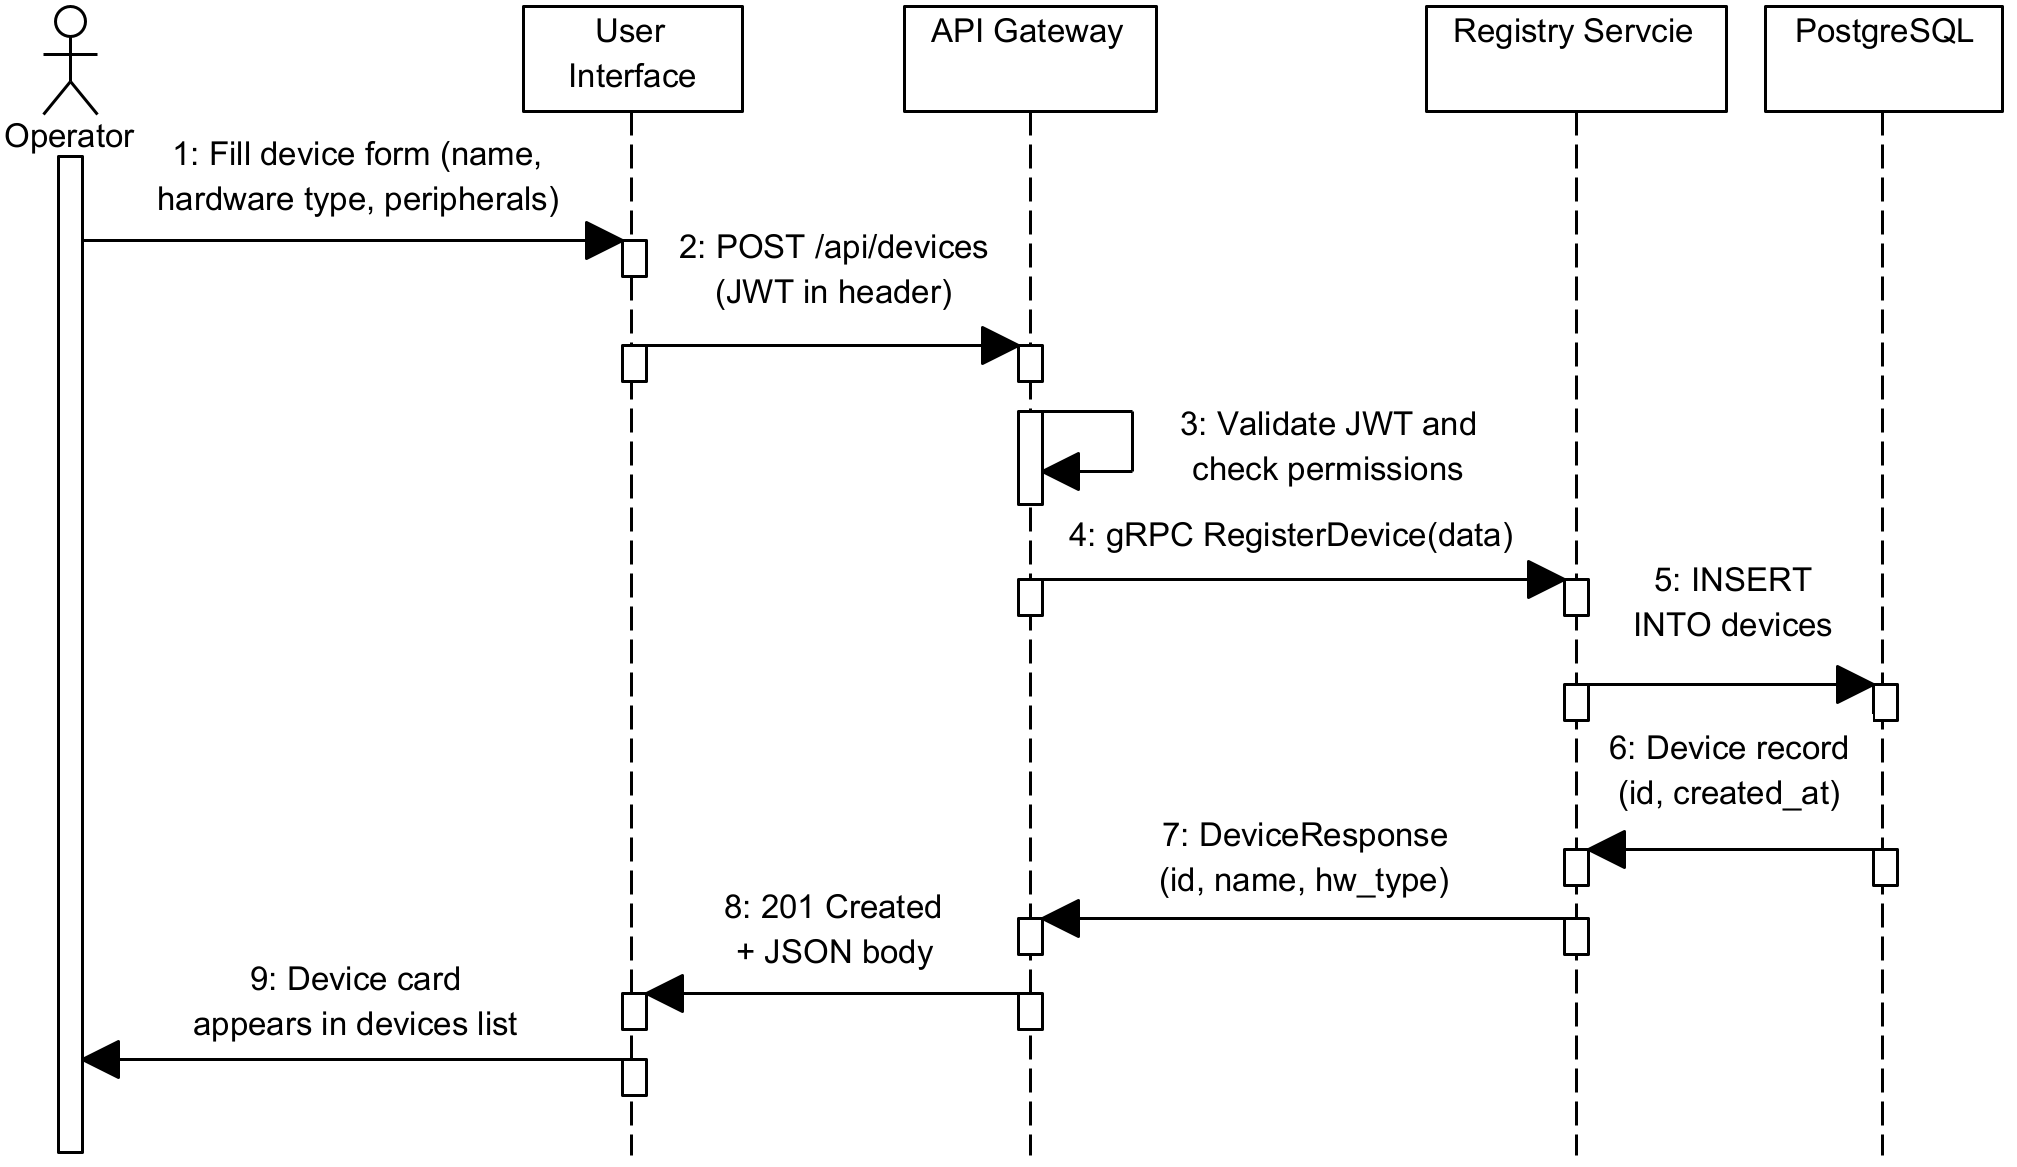
\includegraphics[width=1\linewidth]{images/Device Registration.png}
    \caption{Device Registration Workflow}
    \label{fig:wf_registration}
\end{figure}

\subsubsection{Model Registration}\label{sec:impl:wf:model_registration}

The registration sequence for a PyTorch model begins when an operator uploads the model file (.pt) and enters the corresponding metadata through the frontend interface. Upon receiving this \gls{HTTP} multipart request, the \gls{API} Gateway immediately uploads the model binary directly to the dedicated models bucket in the MinIO object storage.

Next, the \gls{API} Gateway triggers the RegisterModel \gls{gRPC} call on the Registry Service, which inserts a new record with a "pending" status into the PostgreSQL database. To complete the workflow, the \gls{API} Gateway returns a \gls{HTTP} 201 Created response to the frontend, providing the newly registered model's metadata in \gls{JSON} format.

\begin{figure}[H]
    \centering
    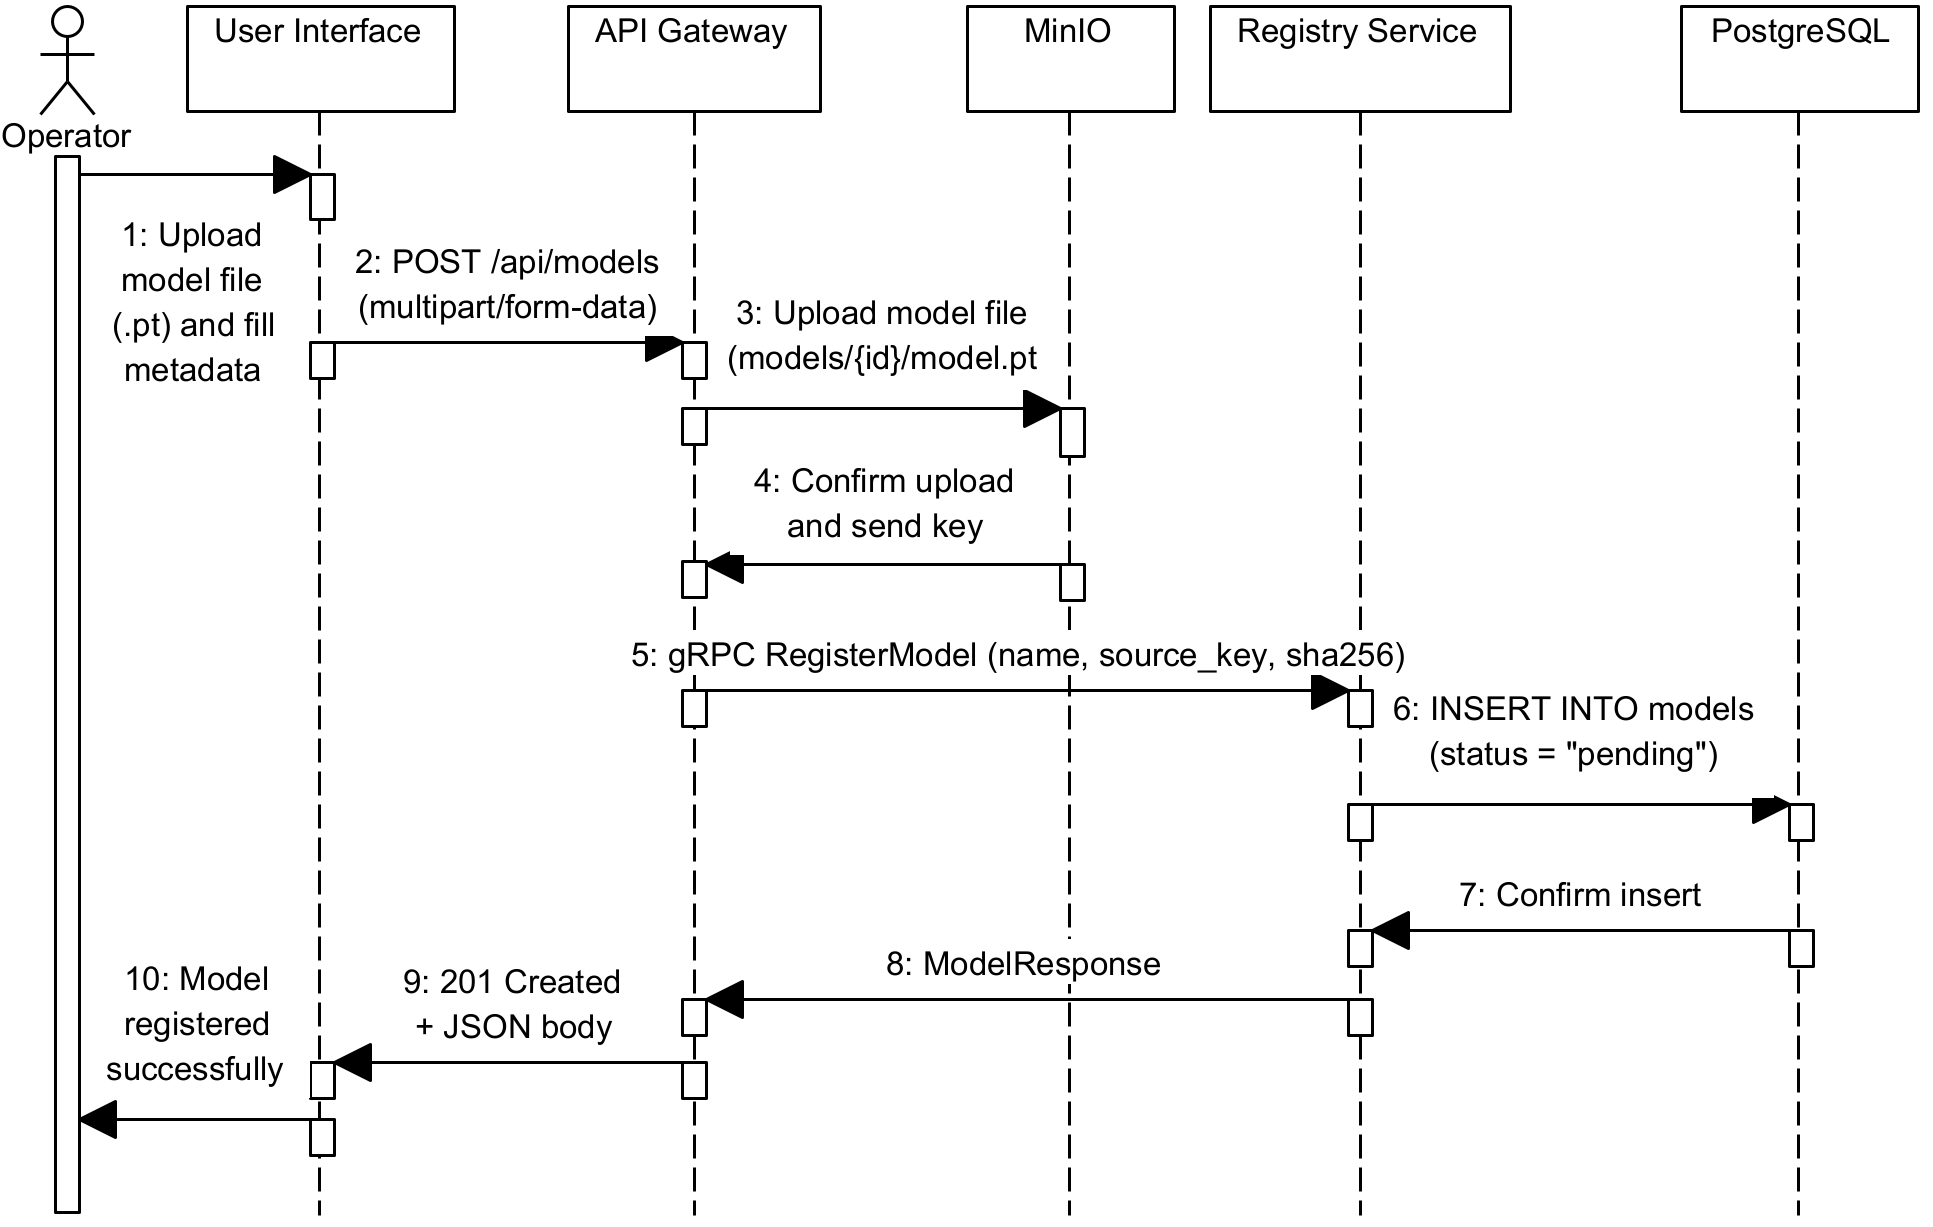
\includegraphics[width=1\linewidth]{images/Model Registration.png}
    \caption{Model Registration Workflow}
    \label{fig:wf_model_registration}
\end{figure}

Importantly, datasets and custom scripts are registered in an analogous manner: datasets are uploaded as \texttt{.zip} files to the \texttt{datasets} MinIO bucket, while custom scripts are uploaded to the \texttt{scripts} bucket, both writing their metadata in PostgreSQL through their respective Registry Service stubs.

\subsubsection{Model Training}\label{sec:impl:wf:training}

Training is an asynchronous pipeline. The operator selects a dataset, a YOLO base architecture, and parameters (epochs, input size, batch size) from the frontend. The \gls{API} Gateway registers the model metadata via the Registry Service and triggers the training through the \gls{MLOps} Service. 

The worker downloads the dataset from MinIO, launches the YOLO subprocess, and streams training logs to Redis in real time for frontend consumption. Upon completion, the trained weights (\texttt{best.pt}) are uploaded to MinIO and the model status transitions to \textit{pending}. 

This status indicates that while the model has been successfully trained and its base weights are available, it has not yet been compiled or optimized for a target edge hardware architecture. The compilation process is deferred until a deployment to a specific device is triggered or an explicit hardware compilation is requested.


\begin{figure}[H]
    \centering
    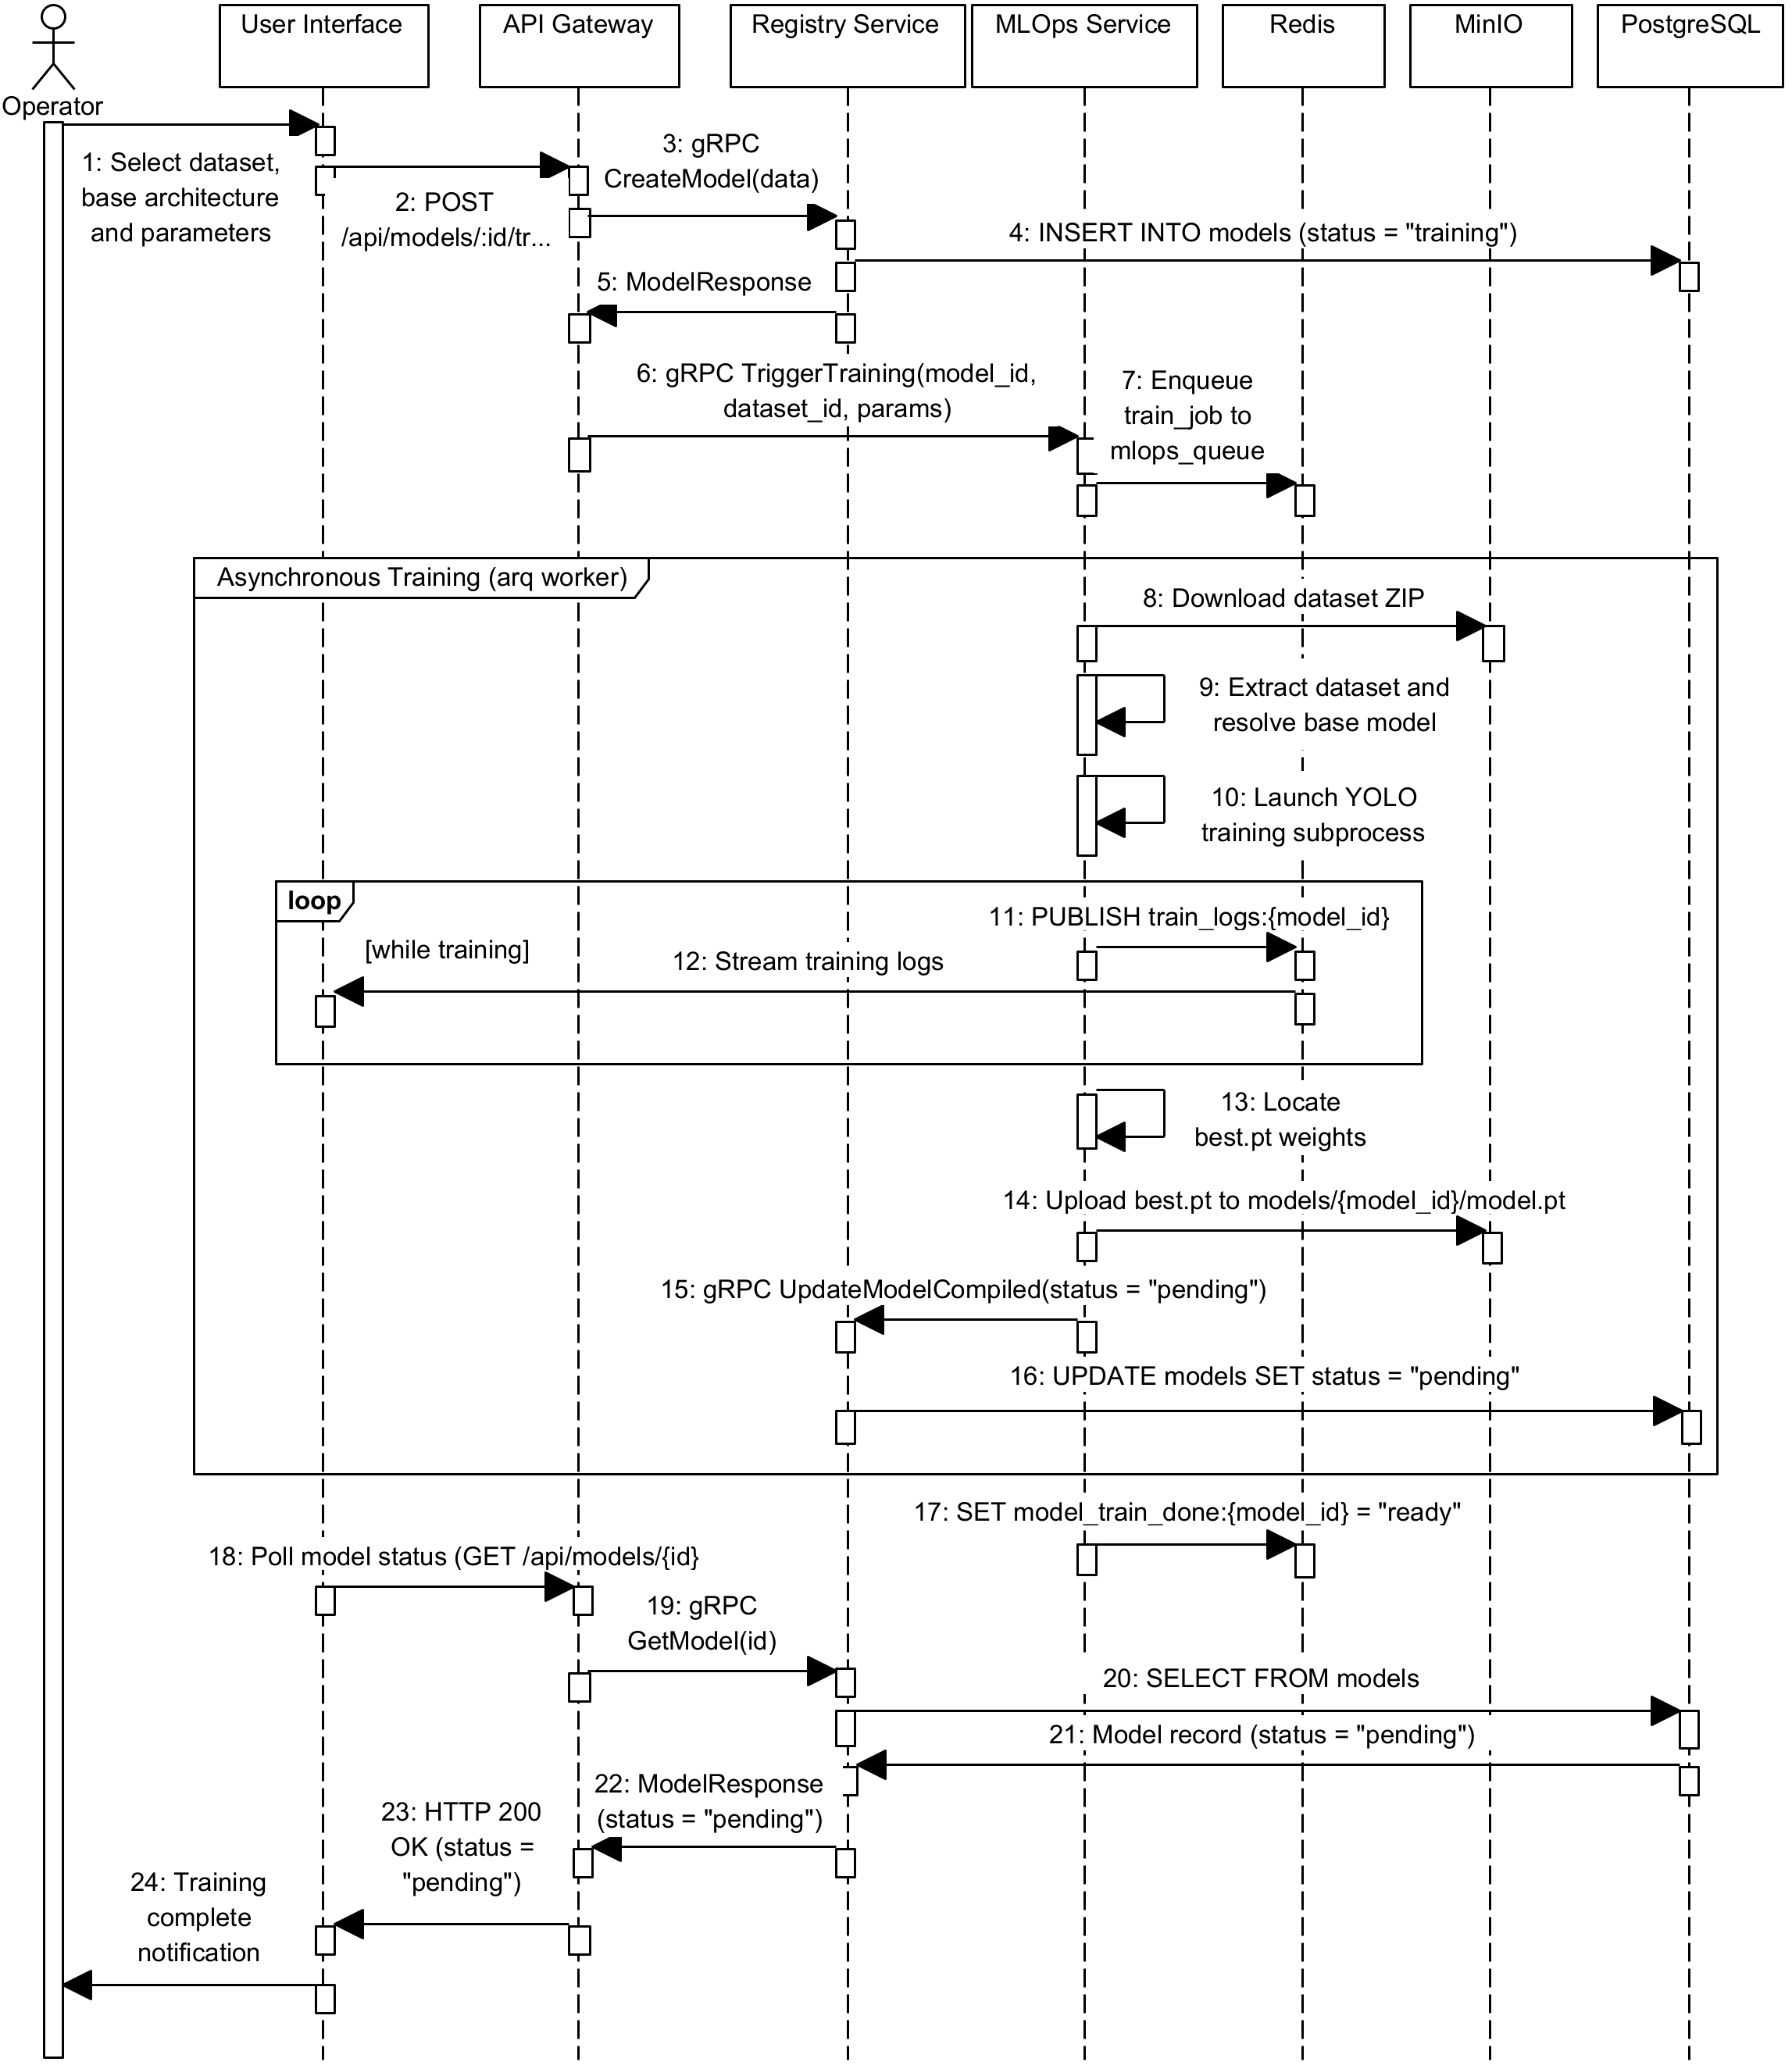
\includegraphics[width=0.95\linewidth]{images/Model Training.png}
    \caption{Model Training Workflow}
    \label{fig:wf_training}
\end{figure}

\subsubsection{Model Retraining}\label{sec:impl:wf:model_retraining}

The model retraining workflow is structurally identical to the model training workflow described in \autoref{sec:impl:wf:training}, with the primary differences being the initialization triggers and the model initialization baseline.

First, rather than being triggered solely by a manual operator request, retraining can be initiated by manual user commands, scheduled periodic events, or automated telemetry-driven drift detection.

Second, during execution, instead of initializing from a standard YOLO base architecture, the asynchronous \gls{MLOps} worker downloads the parent model's trained weights from MinIO to use as a baseline for fine-tuning or transfer learning, along with the newly compiled dataset.


\subsubsection{Model Compilation}\label{sec:impl:wf:compilation}

Once a model is trained, it must be compiled for a specific hardware target before deployment. The compilation job extracts calibration images from the training dataset and invokes the appropriate hardware-specific compiler. The compiled artefact and its SHA-256 checksum are uploaded to MinIO and registered in the database.

\begin{figure}[H]
    \centering
    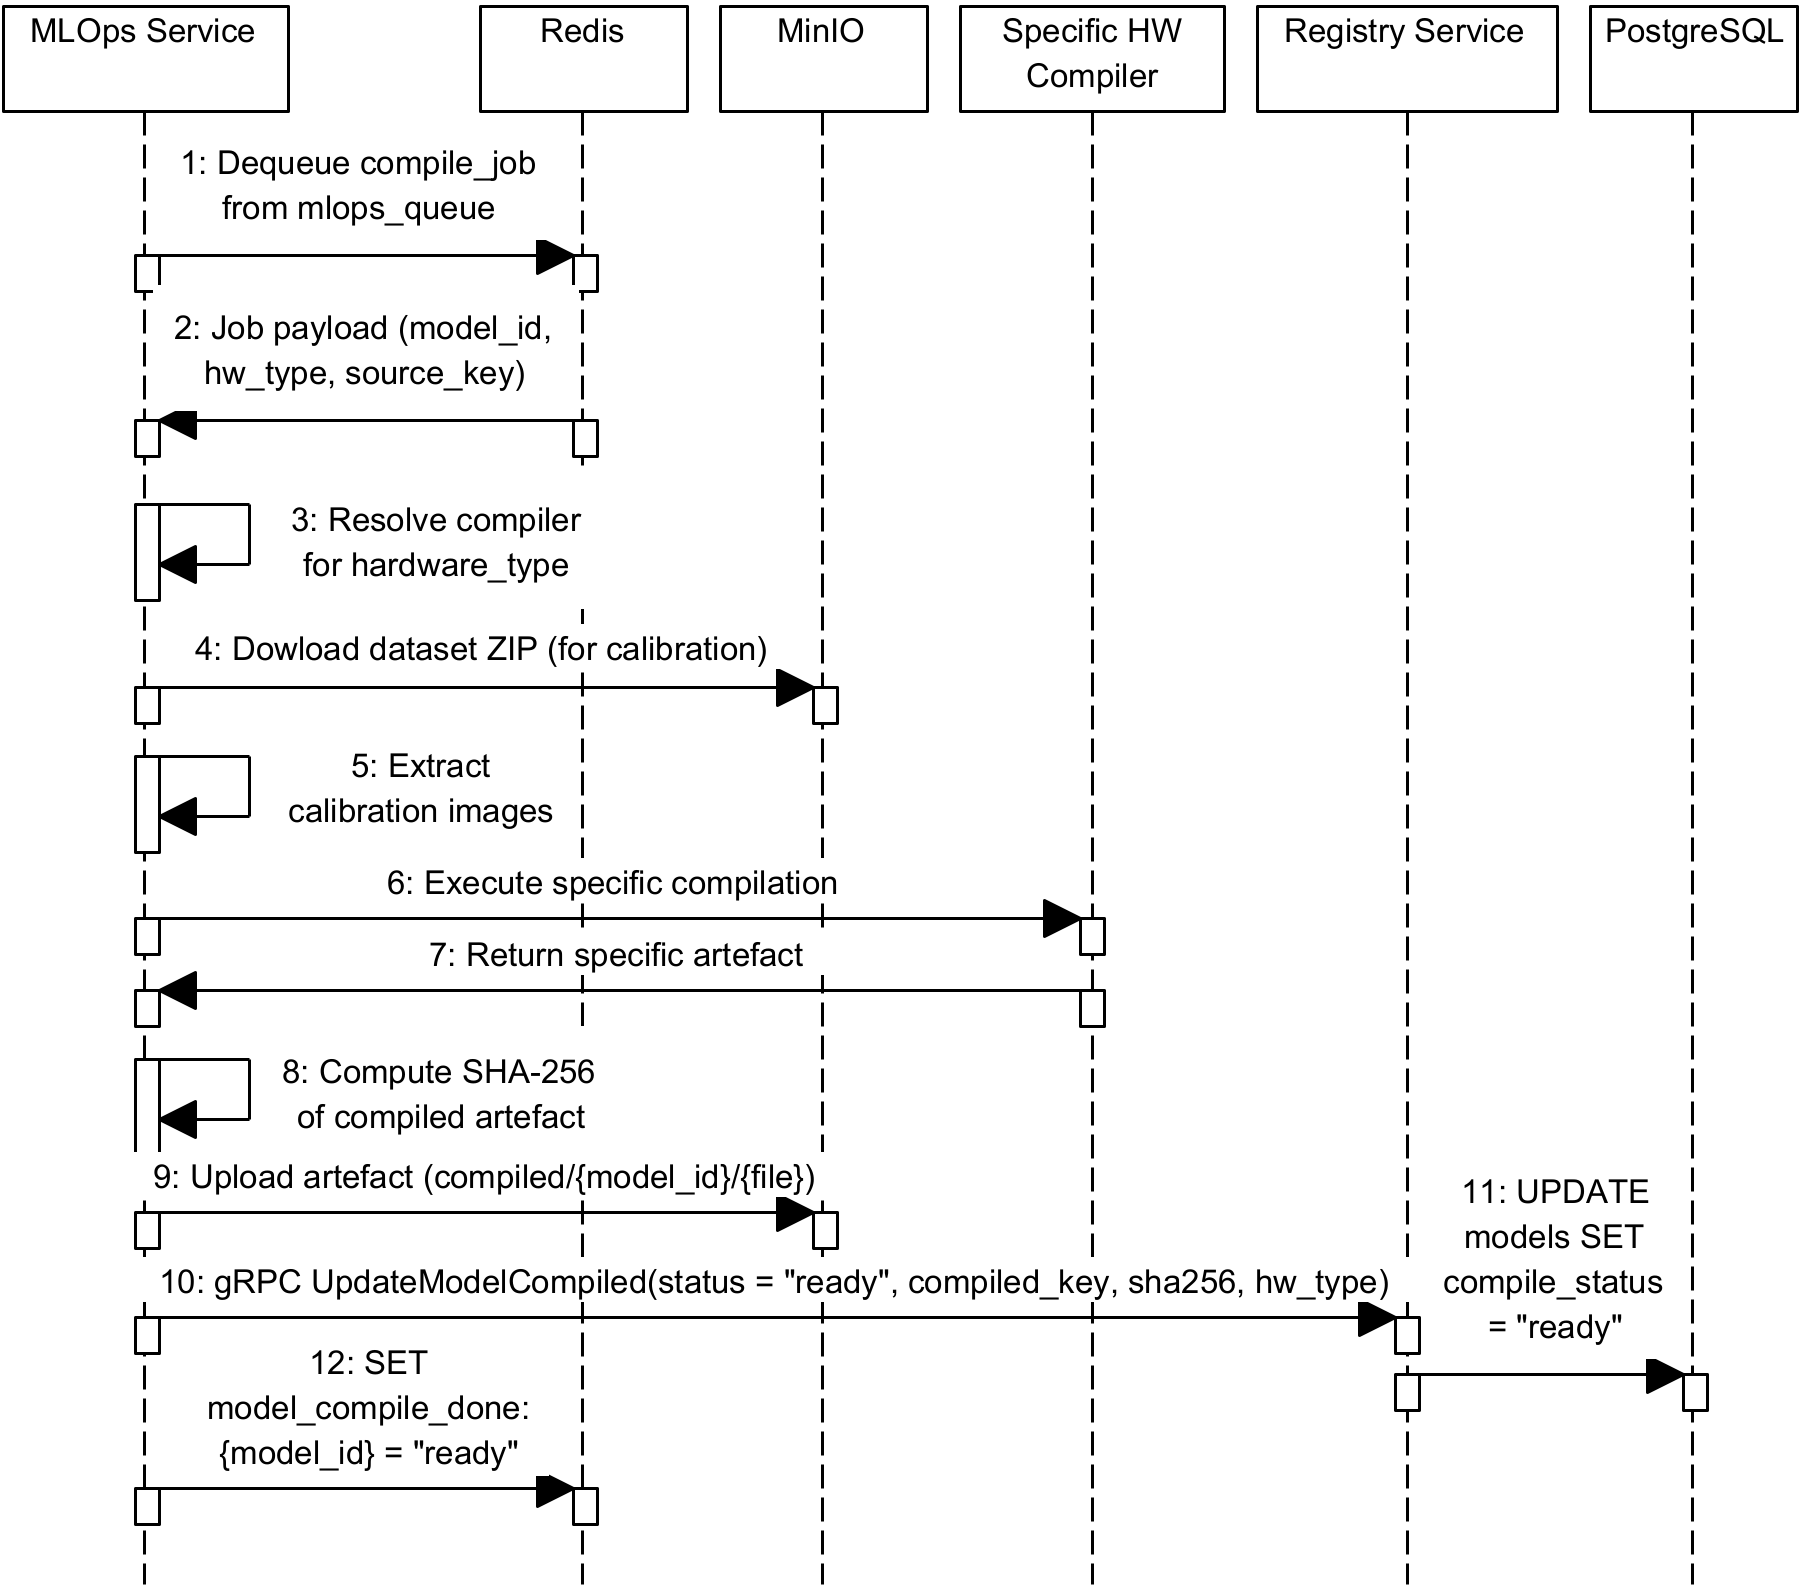
\includegraphics[width=0.9\linewidth]{images/Model Compilation.png}
    \caption{Model Compilation Workflow}
    \label{fig:wf_compilation}
\end{figure}

\subsubsection{\texorpdfstring{\acrshort{OTA}}{OTA} Deployment}\label{sec:impl:wf:deployment}

The deployment pipeline is the most complex workflow in the platform. When a deployment is triggered, the Edge Connector Service checks whether the model is already compiled for the target device's hardware. 

If so, it immediately generates presigned MinIO \glspl{URL} and publishes a \texttt{deploy} command over \gls{MQTT}. Otherwise, it enqueues a background job that first triggers compilation and then waits for the result by polling a Redis key.

On the edge side, the \gls{OTA} Handler downloads the model and script artefacts, verifies their SHA-256 checksums, atomically loads the new model into the \gls{HAL}Backend, and hot-reloads the user script. A \texttt{deploy\_ack} or \texttt{deploy\_failed} event is published back to the platform, which updates the deployment status accordingly.

\begin{figure}[H]
    \centering
    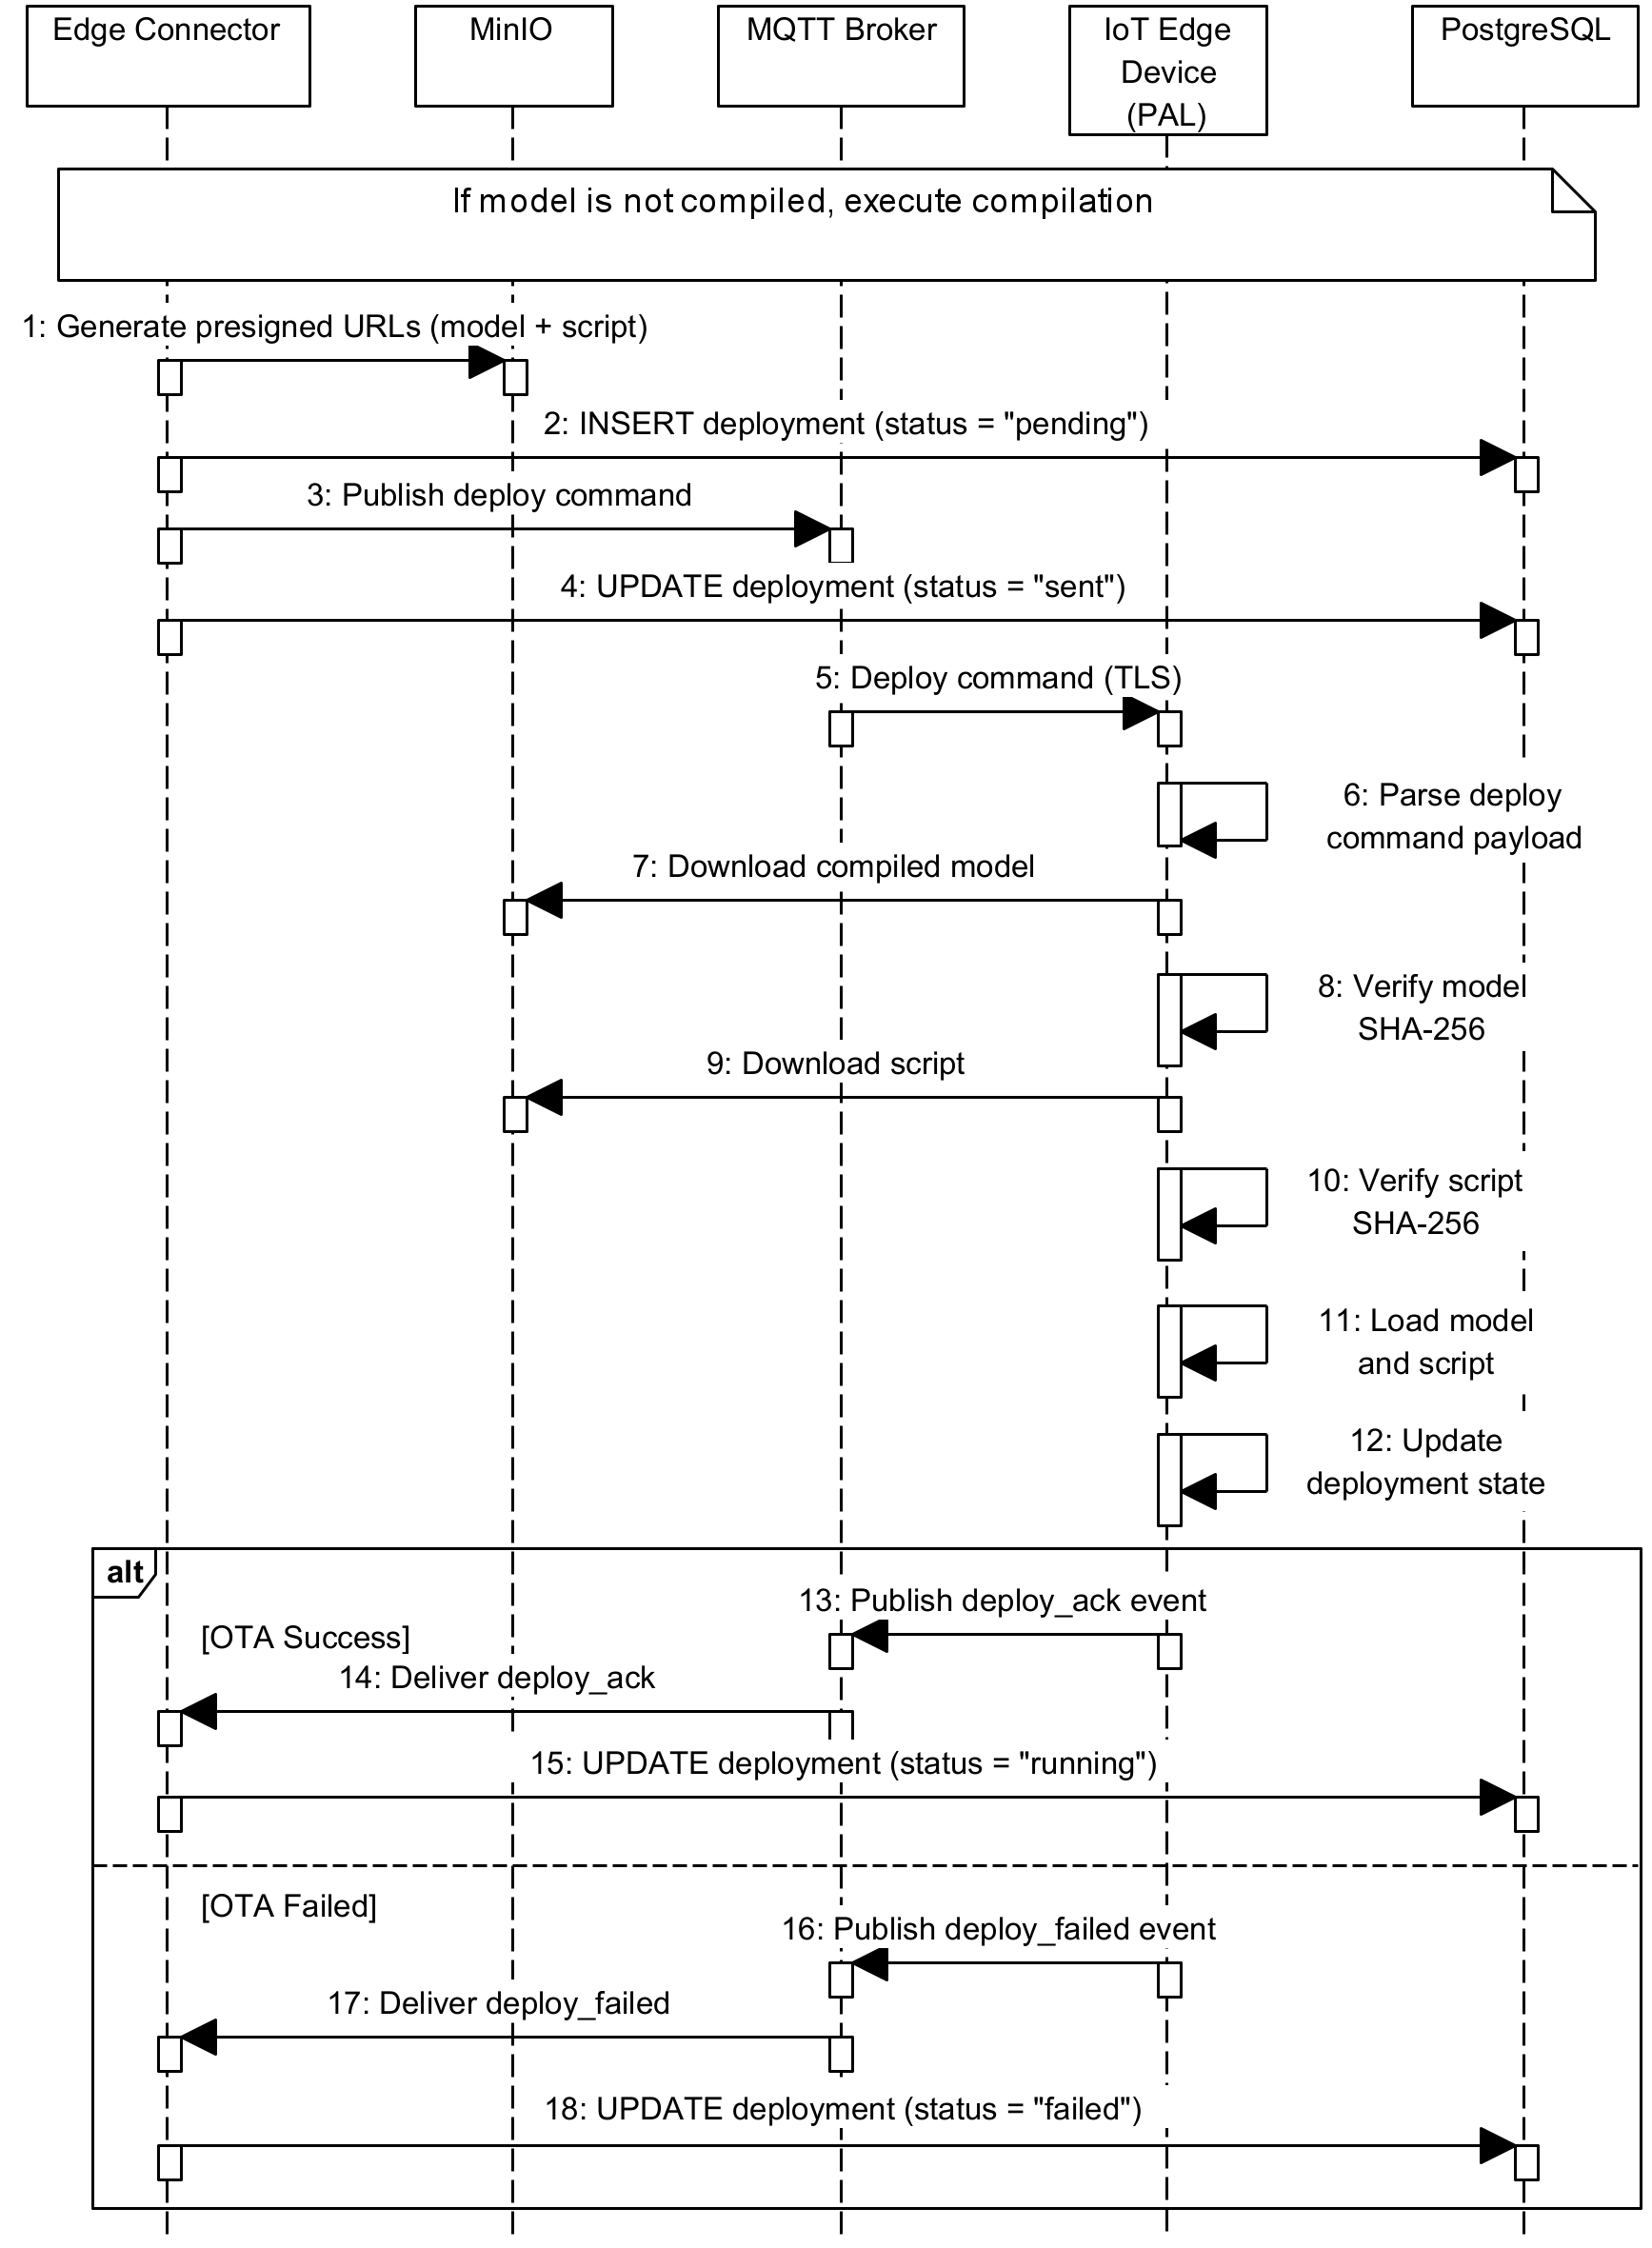
\includegraphics[width=0.9\linewidth]{images/OTA Deployment.png}
    \caption{\acrshort{OTA} Deployment Workflow}
    \label{fig:wf_deployment}
\end{figure}

\subsubsection{Real-Time Inference \& Telemetry Loops}\label{sec:impl:wf:inference}

The Orchestrator runs two concurrent asynchronous loops. The \textbf{inference loop} (100ms interval) runs the custom script. In this example, it captures frames from the primary camera, inferences them through the \gls{HAL}Backend, processes and publishes the results. The Edge Connector Service receives the inference results and stores them in MongoDB.

\begin{figure}[H]
    \centering
    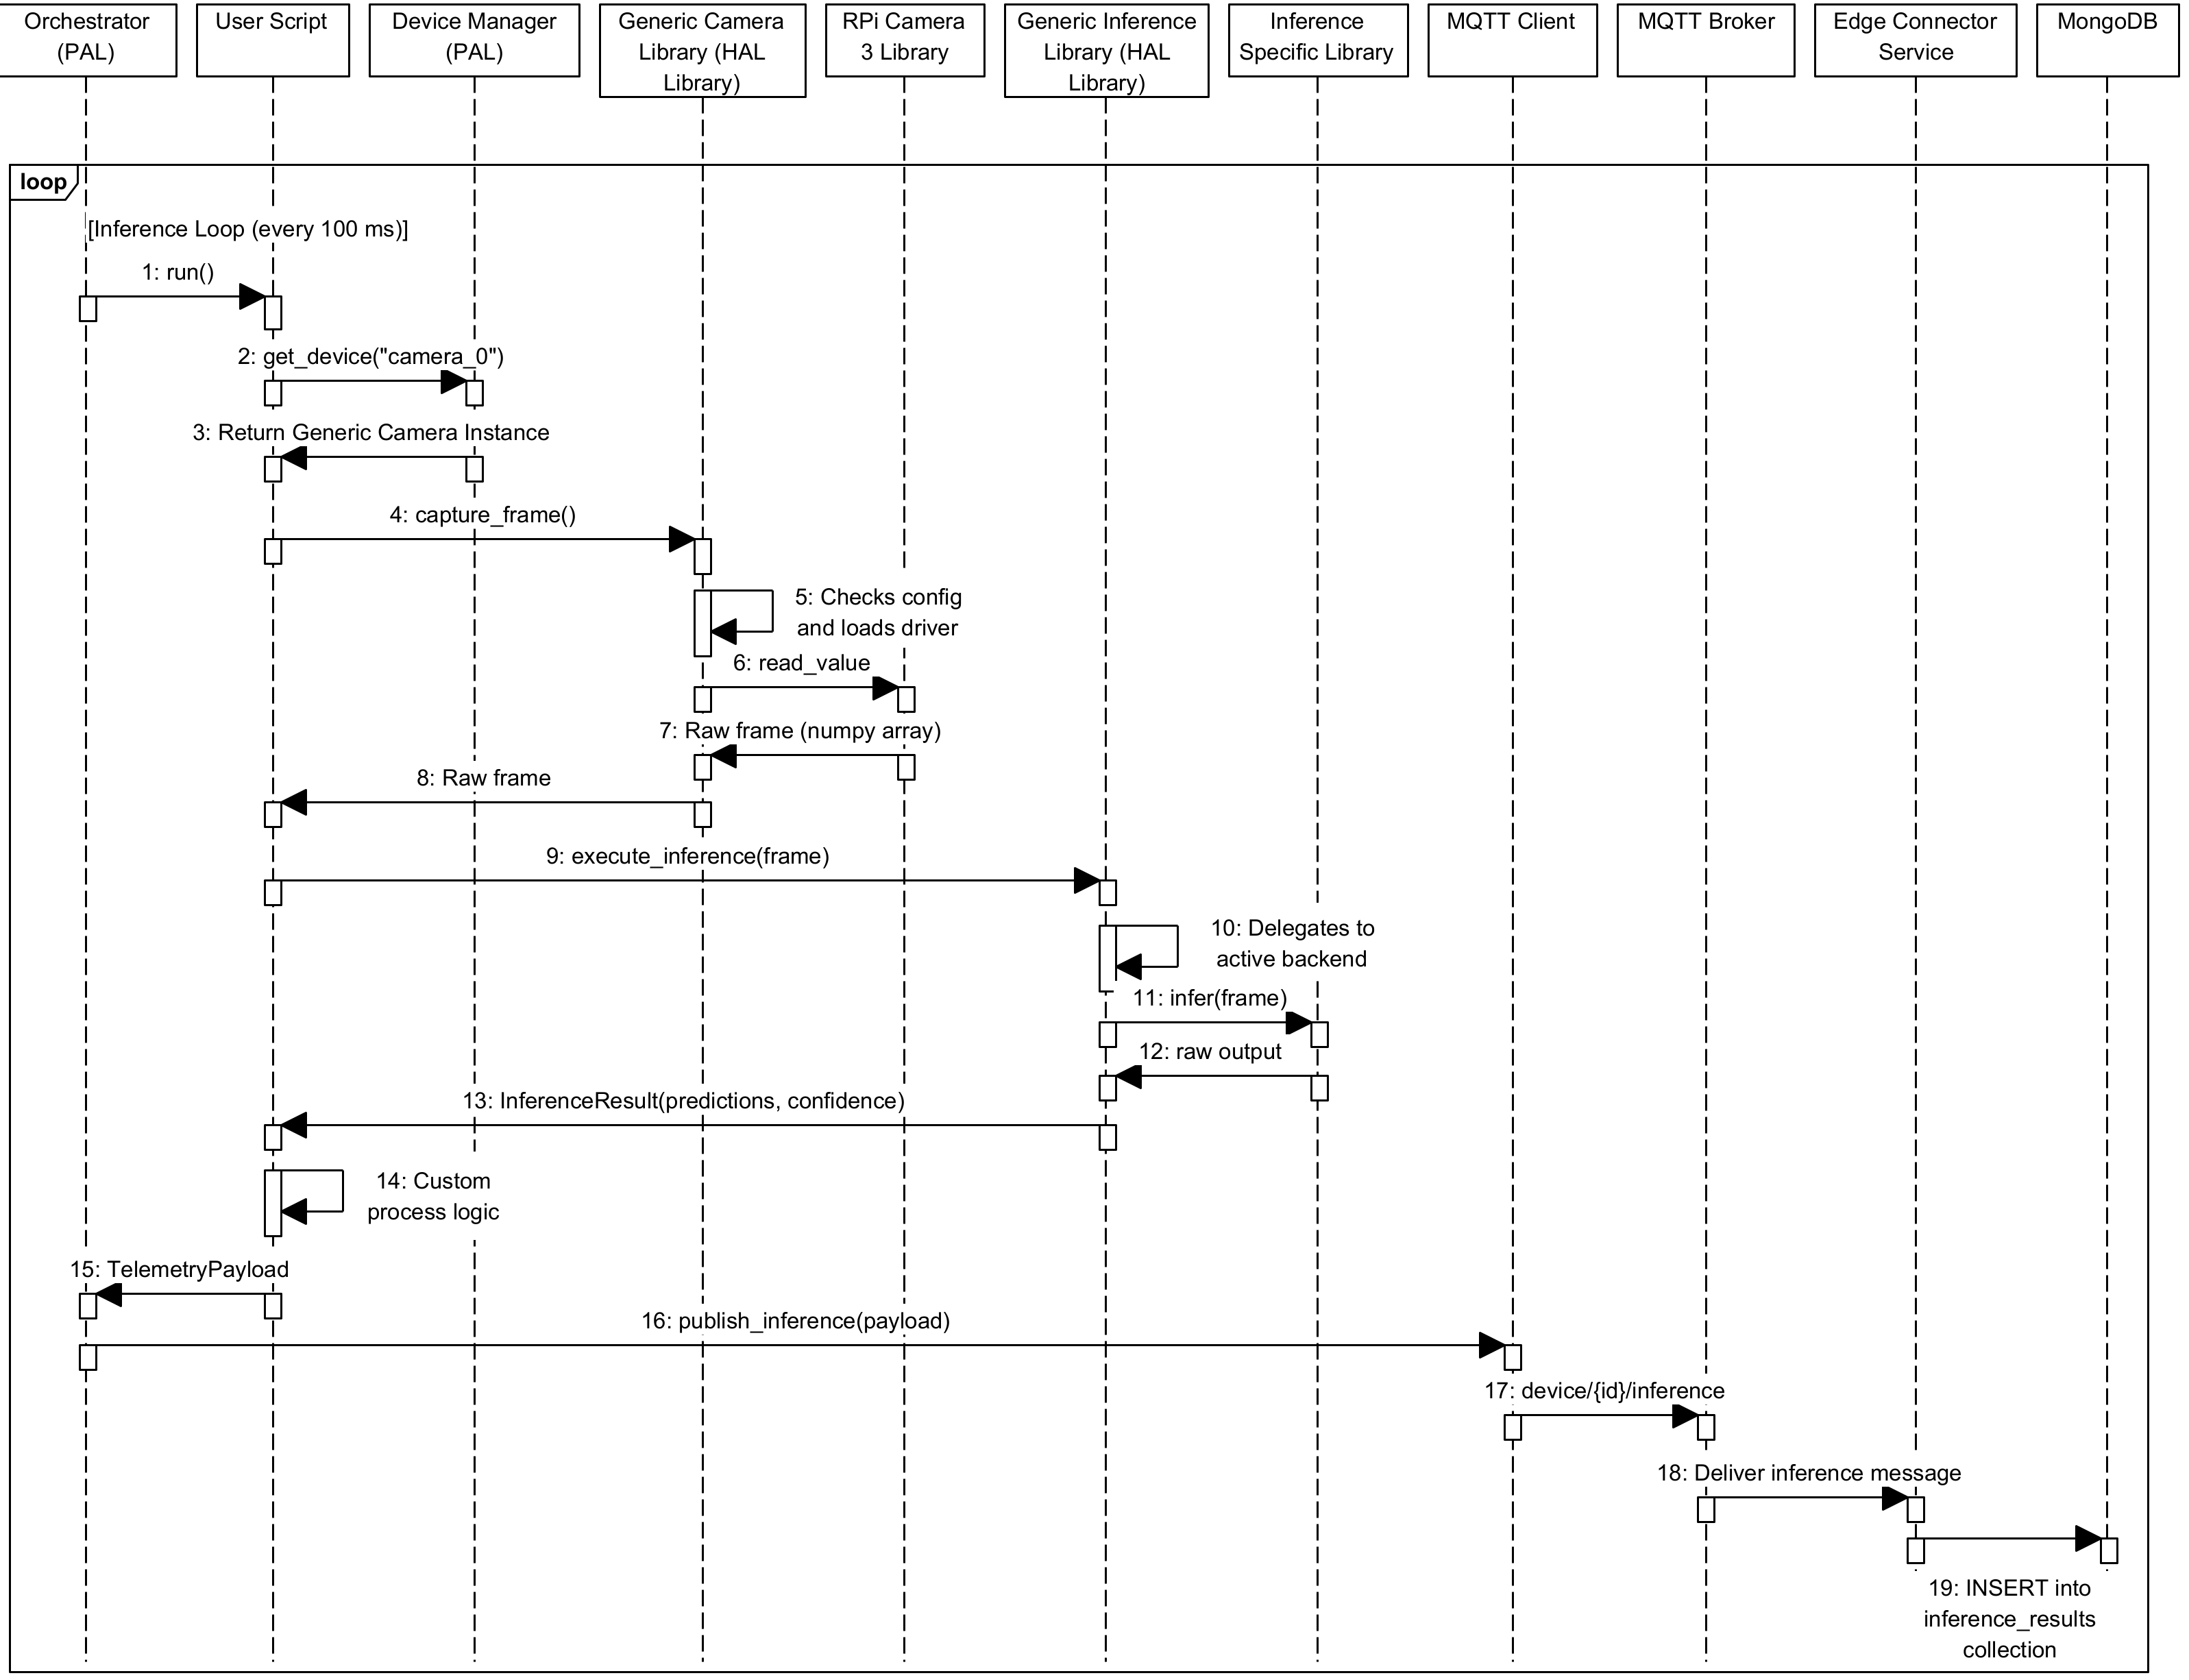
\includegraphics[angle=90,origin=c,height=0.72\textheight]{images/Inference.png}
    \caption{Real-Time Inference Loop Workflow}
    \label{fig:wf_inference}
\end{figure}

The \textbf{telemetry loop} (10s interval) collects system health metrics (\gls{CPU}, \gls{RAM}, temperatures), peripheral states, and the active deployment metadata, publishing a combined payload to \texttt{device/\{id\}/telemetry}. The Edge Connector Service receives the telemetry data updates and saves them in MongoDB and Prometheus.

\begin{figure}[H]
    \centering
    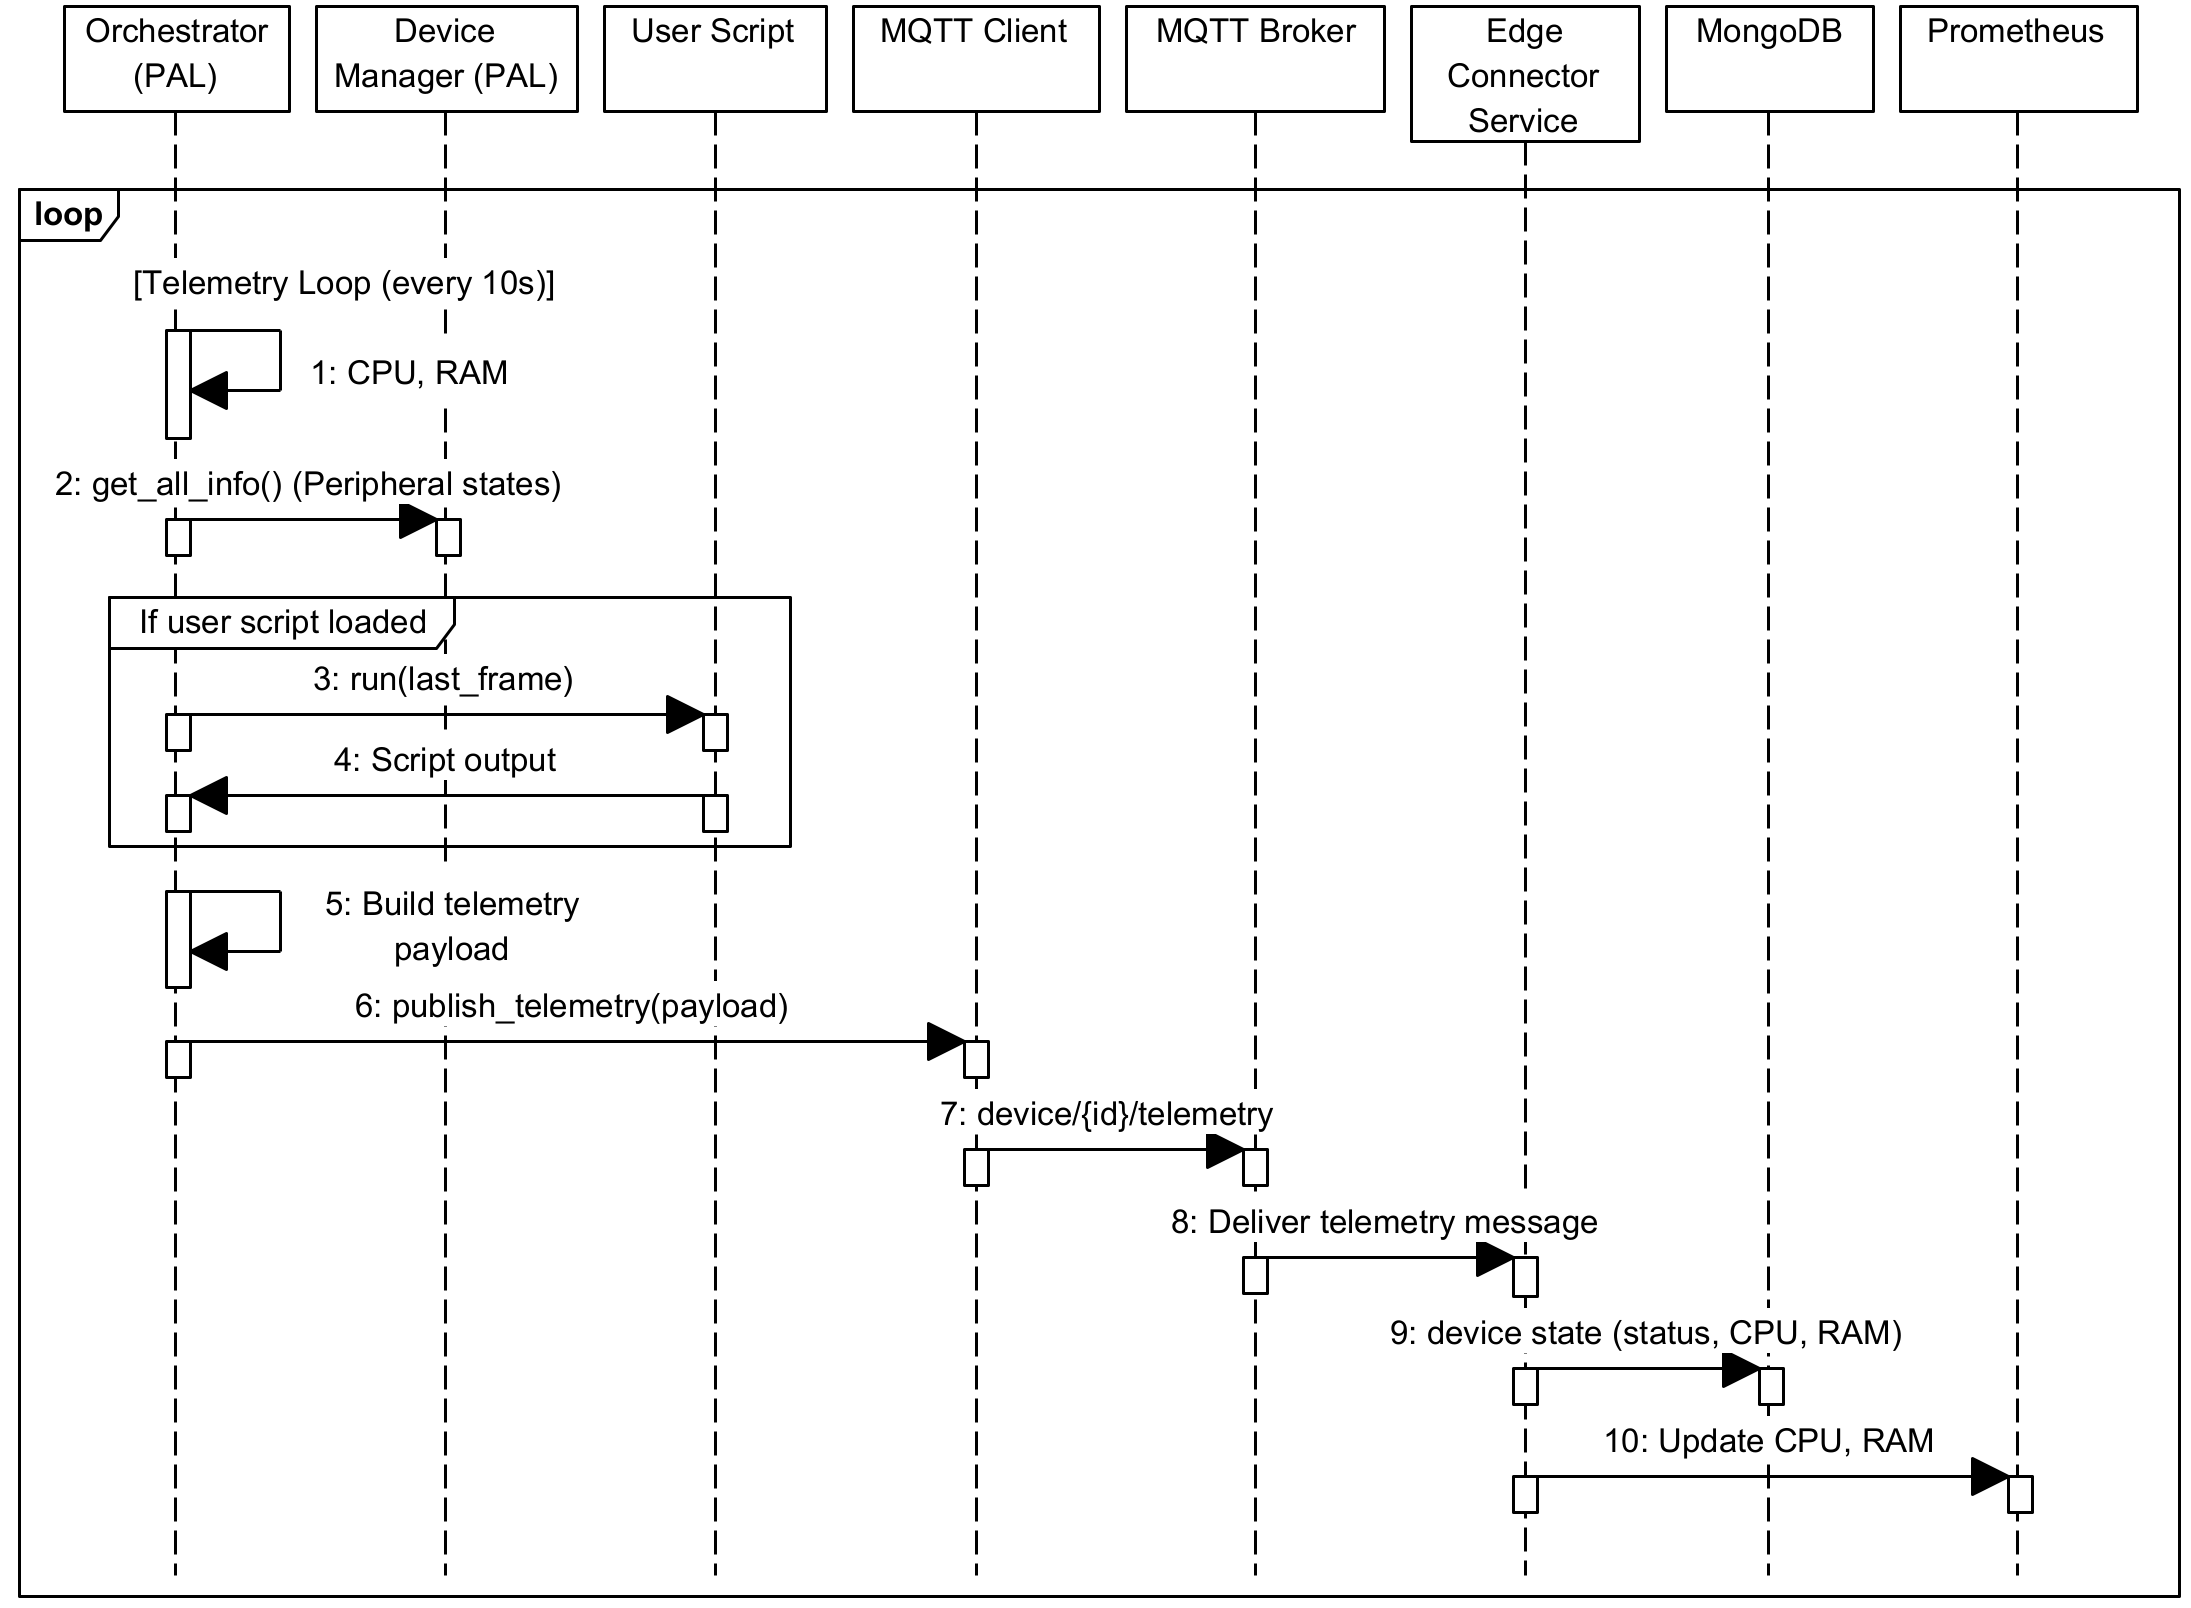
\includegraphics[angle=90,origin=c,height=0.72\textheight]{images/Telemetry.png}
    \caption{Real-Time Telemetry Loop Workflow}
    \label{fig:wf_telemetry}
\end{figure}

\subsubsection{Dynamic Hardware Libraries Sync}\label{sec:impl:wf:libraries}

The platform maintains a set of hardware abstraction libraries that \gls{IoT} Edge devices must keep synchronised. Each telemetry payload includes a \texttt{libraries\_hash} computed from the device's local hardware directory. 

The Edge Connector Service compares this hash against its own platform-side hash. On mismatch, it packages the platform's hardware directory into a ZIP archive, uploads it to MinIO, and publishes an \texttt{update\_libraries} command. 

The edge \gls{OTA} Handler downloads the archive, verifies its integrity, replaces the local hardware directory, and acknowledges the update.

\begin{figure}[H]
    \centering
    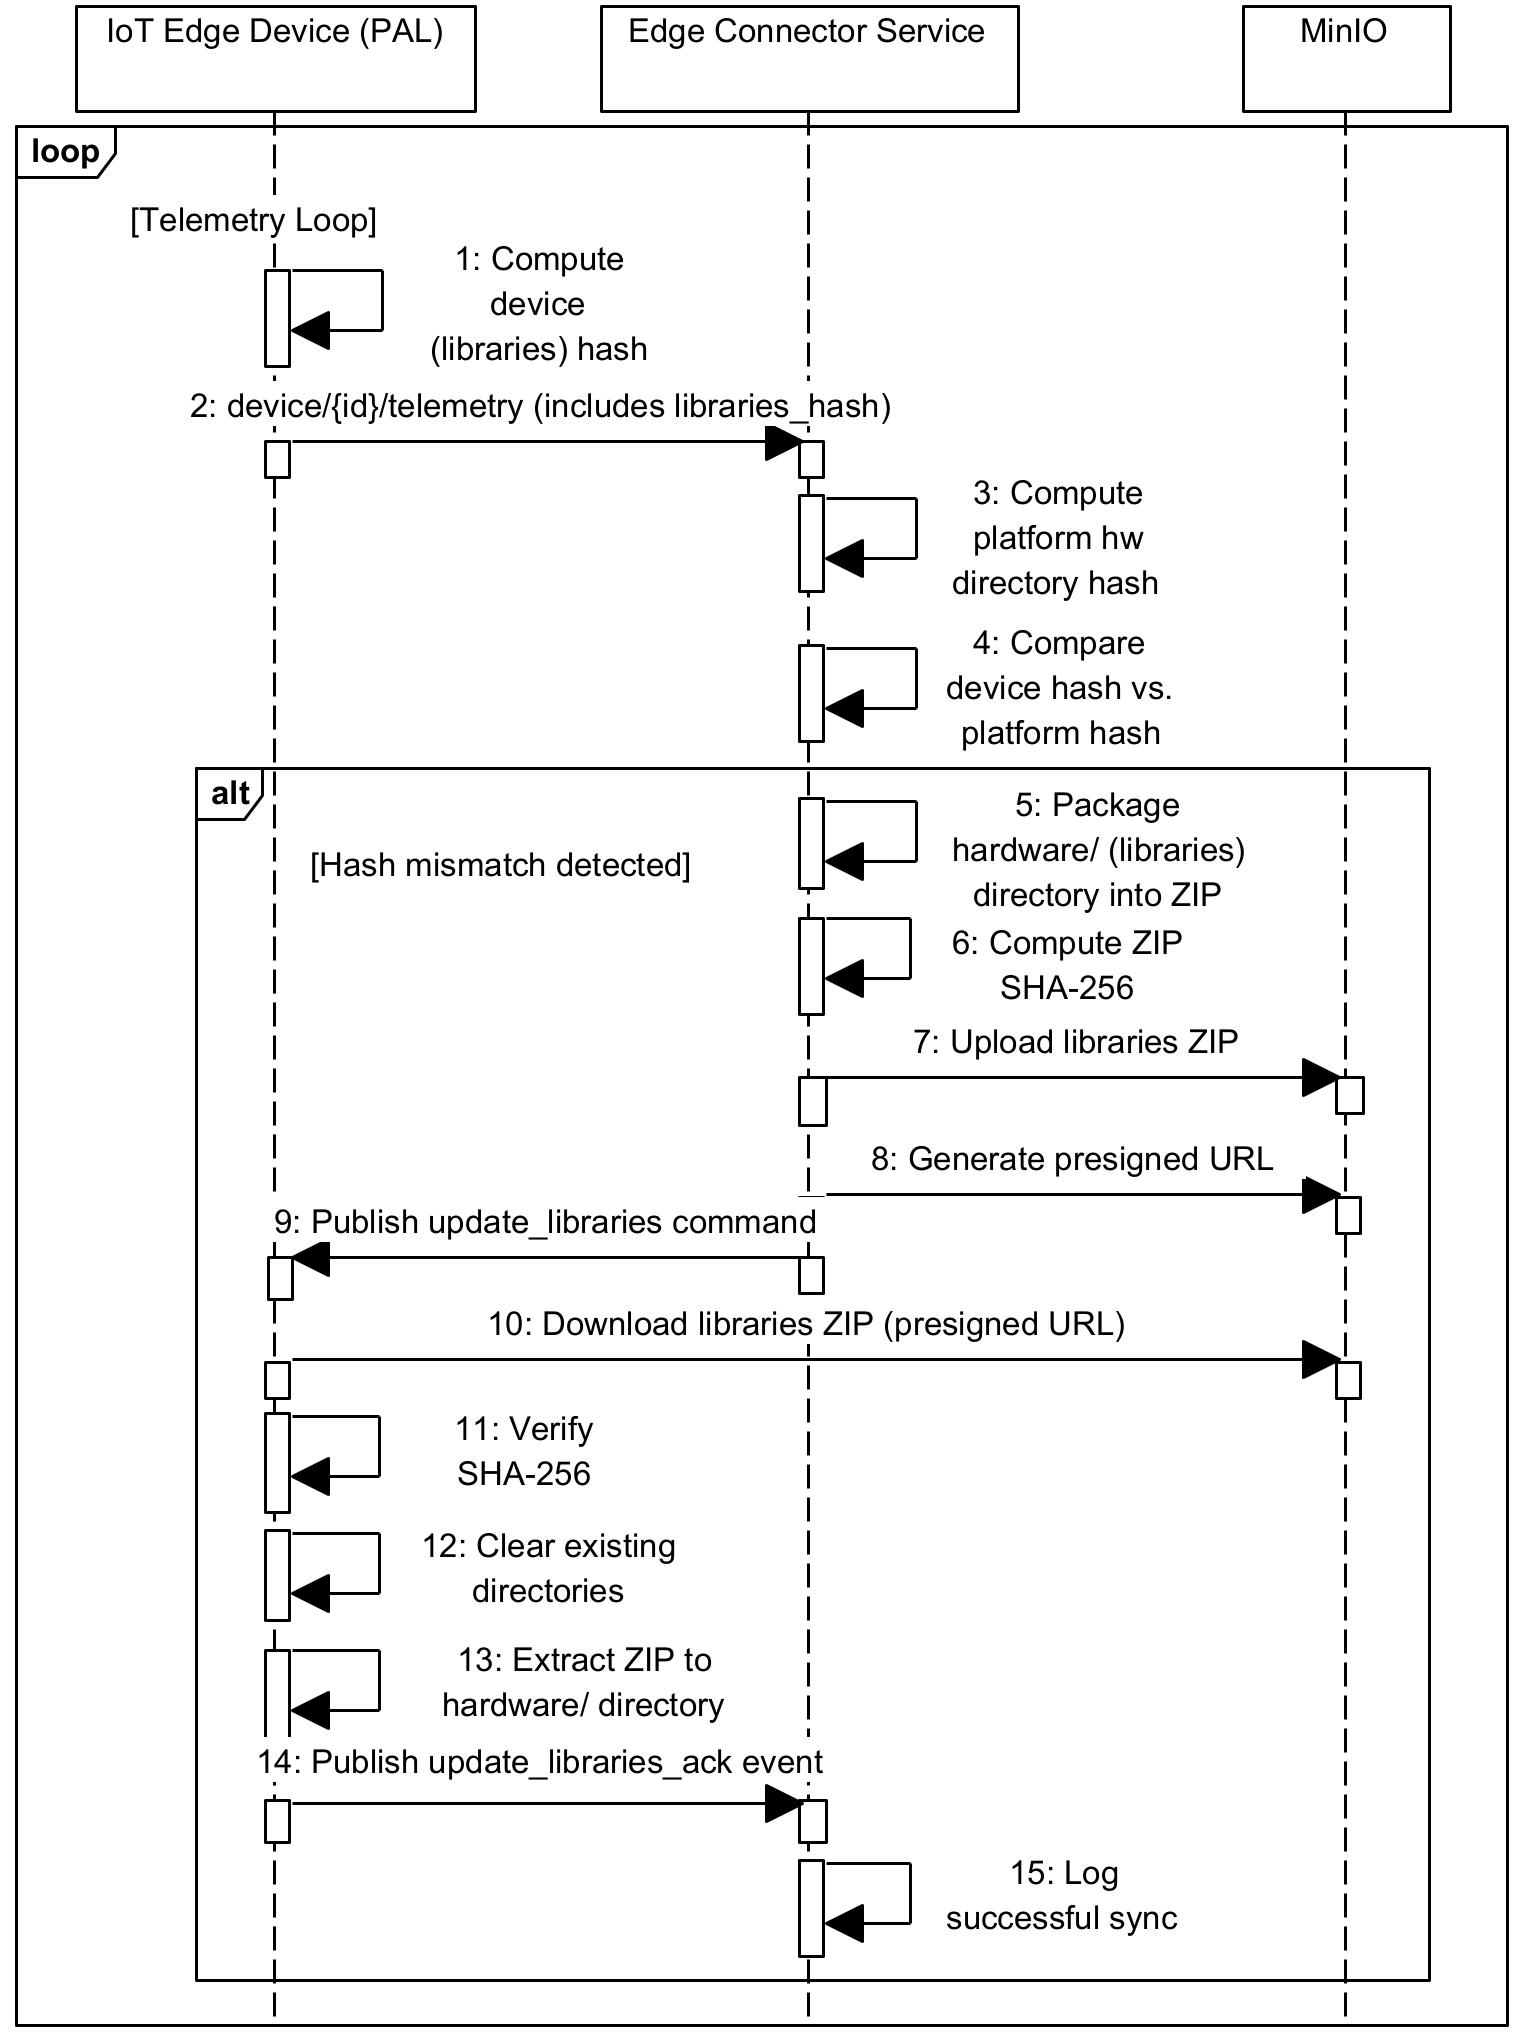
\includegraphics[width=0.79\linewidth]{images/Libraries Sync.png}
    \caption{Dynamic Hardware Libraries Sync Workflow}
    \label{fig:wf_libraries}
\end{figure}

